\documentclass[letterpaper,english,10pt]{article}
\usepackage{%
	amsfonts,%
	amsmath,%	
	amssymb,%
	amsthm,%
	babel,%
	bbm,%
	%biblatex,%
	caption,%
	centernot,%
	color,%
	enumerate,%
	%enumitem,%
	epsfig,%
	epstopdf,%
	etex,%
	fancybox,%
	framed,%
	fullpage,%
	%geometry,%
	graphicx,%
	hyperref,%
	latexsym,%
	mathptmx,%
	mathtools,%
	multicol,%
	pgf,%
	pgfplots,%
	pgfplotstable,%
	pgfpages,%
	proof,%
	psfrag,%
	%subfigure,%	
	tikz,%
	times,%
	ulem,%
	url,%
	xcolor,%
	mathpazo
}

\definecolor{shadecolor}{gray}{.95}%{rgb}{1,0,0}
\usepackage[margin=1in,top=0.75in]{geometry}
\usepackage[mathscr]{eucal}
\usepgflibrary{shapes}
\usepgfplotslibrary{fillbetween}
\usetikzlibrary{%
  arrows,%
  backgrounds,%
  chains,%
  decorations.pathmorphing,% /pgf/decoration/random steps | erste Graphik
  decorations.text,% 
  matrix,%
  positioning,% wg. " of "
  fit,%
  patterns,%
  petri,%
  plotmarks,%
  scopes,%
  shadows,%
  shapes.misc,% wg. rounded rectangle
  shapes.arrows,%
  shapes.callouts,%
  shapes%
}

%\pgfplotsset{compat=newest} %<------ Here
\pgfplotsset{compat=1.11} %<------ Or use this one

\theoremstyle{plain}
\newtheorem{thm}{Theorem}[section]
\newtheorem{lem}[thm]{Lemma}
\newtheorem{prop}[thm]{Proposition}
\newtheorem{cor}[thm]{Corollary}
\newtheorem{clm}[thm]{Claim}

\theoremstyle{definition}
\newtheorem{axiom}[thm]{Axiom}
\newtheorem{defn}[thm]{Definition}
\newtheorem{conj}[thm]{Conjecture}
\newtheorem{exmp}[thm]{Example}
\newtheorem{exerc}[thm]{Exercise}
\newtheorem{assum}[thm]{Assumptions}

\theoremstyle{remark}
\newtheorem{rem}[thm]{Remark}
\newtheorem{note}[thm]{Note}

\newcommand{\Cov}{\operatorname{Cov}}
%\newcommand{\det}{\operatorname{det}}
\newcommand{\Real}{\mathbb{R}}
\newcommand{\tr}{\operatorname{tr}}
%\newcommand{\Var}{\operatorname{Var}}

\DeclareMathOperator{\sign}{sign}
%\renewcommand{\proof}[1]{\begin{proof}#1\end{proof}}
\newcommand{\EQ}[1]{\begin{equation*}#1\end{equation*}}
\newcommand{\EQN}[1]{\begin{equation}#1\end{equation}}
\newcommand{\eq}[1]{\begin{align*}#1\end{align*}}
\newcommand{\meq}[2]{\begin{xalignat*}{#1}#2\end{xalignat*}}
\newcommand{\norm}[1]{\left\lVert#1\right\rVert}
\newcommand{\abs}[1]{\left\lvert#1\right\rvert}
\newcommand{\expect}[1]{\mathbb{E}\left[{#1}\right]}
\newcommand{\prob}[1]{\mathbb{P}\left[{#1}\right]}
\newcommand{\given}{\; \big\vert \;} 
\newcommand{\set}[1]{\left\{#1\right\}} 
\newcommand{\indicator}[1]{\mathbb{1}_{\set{#1}}} 
\newcommand{\inner}[1]{\left\langle#1\right\rangle}
\newcommand{\red}[1]{\textcolor{red}{#1}} 
\newcommand{\E}[1]{\mathbb{E}\left[#1\right]}
\newcommand{\Var}[1]{\operatorname{Var}\left[#1\right]}

\newcommand{\D}{\mathbb{D}}
%\newcommand{\E}{\mathbb{E}}
\newcommand{\N}{\mathbb{N}}
\renewcommand{\P}{\mathbb{P}}
\newcommand{\Q}{\mathbb{Q}}
\newcommand{\R}{\mathbb{R}}
\newcommand{\Z}{\mathbb{Z}}

\newcommand{\bU}{\mathbf{1}}
\newcommand{\bx}{\mathbf{x}}

\newcommand{\cB}{\mathcal{B}}
\newcommand{\cC}{\mathcal{C}}
\newcommand{\cD}{\mathcal{D}}
\newcommand{\cF}{\mathcal{F}}
\newcommand{\cG}{\mathcal{G}}
\newcommand{\cH}{\mathcal{H}}
\newcommand{\cO}{\mathcal{O}}
\newcommand{\cT}{\mathcal{T}}
\newcommand{\cX}{\mathcal{X}}
\newcommand{\cY}{\mathcal{Y}}

\newcommand{\sA}{\mathscr{A}}
\newcommand{\sB}{\mathscr{B}}
\newcommand{\sC}{\mathscr{C}}
\newcommand{\sD}{\mathscr{D}}
\newcommand{\sE}{\mathscr{E}}
\newcommand{\sF}{\mathscr{F}}
\newcommand{\sG}{\mathscr{G}}
\newcommand{\sH}{\mathscr{H}}
\newcommand{\sL}{\mathscr{L}}
\newcommand{\dO}{\mathscr{O}}
\newcommand{\sS}{\mathscr{S}}
\newcommand{\sT}{\mathscr{T}}
\newcommand{\sX}{\mathscr{X}}
\newcommand{\sY}{\mathscr{Y}}
\newcommand{\sZ}{\mathscr{Z}}

% Debug
\newcommand{\todo}[1]{\begin{color}{blue}{{\bf~[TODO:~#1]}}\end{color}}

% a few handy macros

\renewcommand{\le}{\leqslant}
\renewcommand{\ge}{\geqslant}
\newcommand\matlab{{\sc matlab}}
\newcommand{\goto}{\rightarrow}
\newcommand{\bigo}{{\mathcal O}}
%\newcommand{\half}{\frac{1}{2}}
%\newcommand\implies{\quad\Longrightarrow\quad}
\newcommand\reals{{{\rm l} \kern -.15em {\rm R} }}
\newcommand\complex{{\raisebox{.043ex}{\rule{0.07em}{1.56ex}} \hskip -.35em {\rm C}}}


% macros for matrices/vectors:

% matrix environment for vectors or matrices where elements are centered
\newenvironment{mat}{\left[\begin{array}{ccccccccccccccc}}{\end{array}\right]}
\newcommand\bcm{\begin{mat}}
\newcommand\ecm{\end{mat}}

% matrix environment for vectors or matrices where elements are right justifvied
\newenvironment{rmat}{\left[\begin{array}{rrrrrrrrrrrrr}}{\end{array}\right]}
\newcommand\brm{\begin{rmat}}
\newcommand\erm{\end{rmat}}

% for left brace and a set of choices
%\newenvironment{choices}{\left\{ \begin{array}{ll}}{\end{array}\right.}
\newcommand\when{&\text{if~}}
\newcommand\otherwise{&\text{otherwise}}
% sample usage:
%  \delta_{ij} = \begin{choices} 1 \when i=j, \\ 0 \otherwise \end{choices}


% for labeling and referencing equations:
\newcommand{\eql}{\begin{equation}\label}
\newcommand{\eqn}[1]{(\ref{#1})}
% can then do
%  \eql{eqnlabel}
%  ...
%  \end{equation}
% and refer to it as equation \eqn{eqnlabel}.  


% some useful macros for finite difference methods:
\newcommand\unp{U^{n+1}}
\newcommand\unm{U^{n-1}}

% for chemical reactions:
\newcommand{\react}[1]{\stackrel{K_{#1}}{\rightarrow}}
\newcommand{\reactb}[2]{\stackrel{K_{#1}}{~\stackrel{\rightleftharpoons}
   {\scriptstyle K_{#2}}}~}


\makeatletter
\def\th@plain{%
  \thm@notefont{}% same as heading font
  \itshape % body font
}
\def\th@definition{%
  \thm@notefont{}% same as heading font
  \normalfont % body font
}
\makeatother
\date{}

\usepackage{bm}
\graphicspath{{./Figures/}}
%opening
\title{Lecture-09: The Curie-Weiss Model, and a Word on Combinatorial Optimization}
\author{Author: V. Arvind Rameshwar}

\begin{document}
\maketitle
\section{The Curie-Weiss (or Mean-Field) Model}

Last lecture, we looked at the Ising model, in which the $N$-fold configuration space, $\sX_{N}$, was a set of points on a $d$-dimensional lattice, i.e., 
\EQ{
\sX_{N} = \{-1,+1\}^{\mathbb{L}}, \text{ for } \mathbb{L}=\{1,2,\ldots,L\}^{d}.
}
Further, the energy function for a configuration $\bm{\sigma}\in \sX_{N}$ was given by:
\begin{equation*}
    E(\bm{\sigma}) = -\sum_{i\sim j}\sigma_{i}\sigma_j - \sum_{i=1}^{N}B\sigma_i,
\end{equation*}
where $i\sim j$ indicates that the co-ordinate $i$ is adjacent to the co-ordinate $j$, for $i,j\in \mathbb{L}$. Note that the summation in the first term counts the product, $\sigma_i\sigma_j$, for $i\sim j$ exactly once.
We shall now look at yet another setting---the \textbf{Curie-Weiss} model.
As before, the configuration space, $\sX$, is the set $\{-1,+1\}$, and $\sX_{N}$ denotes the $N$-fold Cartesian product of $\sX$ with itself. Let $\bm{\sigma} = (\sigma_1,\ldots,\sigma_N)\in \sX_{N}$, with $\sigma_i \in \{-1,+1\}$, for $i\in [N]$. Then, the energy function, $E(\bm{\sigma})$, for the Curie-Weiss model is:
\begin{equation}\label{energyeq}
E(\bm{\sigma}) = \frac{-1}{2N}\left(\sum_{i}\sum_{j\neq i}\sigma_i\sigma_j\right) - B\sum_{i=1}^{N}\sigma_i,
\end{equation}
where $B$ represents the external magnetic field, as before.
\begin{rem}
The Curie-Weiss model is an example of the more general Mean-Field model.
\end{rem}
Analogous to the notion of average magnetization (defined earlier), we introduce the following definition:
\begin{defn}(Empirical Magnetization)
For a configuration $\bm{\sigma}=(\sigma_1,\ldots,\sigma_N)\in \sX_{N}$, the empirical (or instantaneous) magnetization is given by:
\begin{equation*}
    m(\bm{\sigma}) = \frac{1}{N}\sum_{i=1}^{N}\sigma_i.
\end{equation*}
\end{defn}
An immediate observation is that $\inner{m(\bm{\sigma})} = \frac{1}{N}\sum_{i=1}^{N}\inner{\sigma_i} = M_{N}(\beta,B)$.
Modulo this definition, we can recast the expression for the energy function, in the following form:
\begin{equation*}
    E(\bm{\sigma}) = \left(\frac{N}{2} - \frac{N}{2}(m(\bm{\sigma}))^{2}\right) - BNm(\bm{\sigma}).
\end{equation*}
The expression follows from the facts that:
\begin{align*}
    \frac{-1}{2N}\left(\sum_{i}\sum_{j\neq i}\sigma_i\sigma_j\right) &= \frac{-1}{2N}\left(\sum_{i=1}^{N}\sigma_{i}\sum_{j=1}^{N}\sigma_j - \sum_{i=1}^{N}\sigma_i^{2}\right)\\
    &= \frac{N}{2} - \frac{N}{2}(m(\bm{\sigma}))^{2}\\
    \text{and }-B\sum_{i=1}^{N}\sigma_i &= -BNm(\bm{\sigma}).
\end{align*}
Hereinafter, we shorten $m(\bm{\sigma})$ to $m$, as the argument is implicit.
With this in place, we can write the partition function as
\begin{align*}
    Z_N(\beta,B) &= e^{-N\beta/2}\sum_{\bm{\sigma}}e^{\beta Nm^{2}/2 + \beta BNm}\\
    &\stackrel{(a)}{=}e^{-N\beta/2}\sum_{m}{N\choose N(m+1)/2} e^{\beta Nm^{2}/2 + \beta BNm}\\
    &\stackrel{.}{=}_{N}e^{-N\beta/2}\sum_{m}e^{N\sH((m+1)/2)} e^{\beta Nm^{2}/2 + \beta BNm}
\end{align*}
where equation (a) follows from the observation that the number of positive spins in $\bm{\sigma}$ is $N(m+1)/2$. Moreover, we use $\sH(.)$ to represent the binary entropy function, expressed in nats.

Further approximation in the limit of large $N$ leads us to:
\begin{equation}\label{Zeq}
    Z_N(\beta,B)\stackrel{.}{=}_{N} \int_{-1}^{1}e^{N\phi_{mf}(m;\beta,B)}dm,
\end{equation}
where
\begin{equation}\label{phieq}
    \phi_{mf}(m;\beta,B) := \frac{-\beta}{2}(1-m^{2})+\beta Bm + \sH(\frac{m+1}{2}).
\end{equation}
The largest contribution to the integral in \eqref{Zeq} comes from the largest exponent, and hence, the free energy density,
\begin{equation*}
    \phi(\beta,B) = \sup_{m\in [-1,1]} \phi_{mf}(m;\beta,B).
\end{equation*}
\subsection{Analysis of $\phi_{mf}(m;\beta,B)$}
In what follows, we shall take a look at how $\phi_{mf}$ behaves on varying $\beta$ and $m$.
To obtain the point of maximum, $m^{*}$, of $\phi_{mf}(.)$, we note from \eqref{phieq} that:
\begin{equation*}
    0 = \frac{\partial \phi_{mf}(m;\beta,B)}{\partial m}\Bigr|_{\substack{m=m^{*}}} = \beta m^{*} +\beta B + \frac{1}{2}log\left(\frac{2}{m^{*}+1}-1\right),
\end{equation*}
which yields:
\begin{equation}\label{meq}
    m^{*} = \tanh(\beta m^{*} + \beta B)
\end{equation}
Now that we have calculated the point of maximum of $\phi_{mf}(m;\beta,B)$, we seek to characterize the variation of $\phi(\beta,B)=\phi_{mf}(m^{*};\beta,B)$, with $\beta$.
From \eqref{meq}, it is easy to arrive at the fact that
\begin{equation}\label{parteq}
    \frac{\partial m^{*}}{\partial \beta} = \frac{(1-(m^{*})^{2})(B+m^{*})}{1-\beta(1-(m^{*})^{2})}
\end{equation}
As a simplifying assumption, we take $B=0$. Let us denote by $g(\beta)$, the partial derivative of $\phi(\beta,0)$ with respect to $\beta$, i.e.,
\begin{equation*}
    g(\beta) = \frac{\partial \phi(\beta,0)}{\partial \beta} = \frac{\partial \phi_{mf}(m^{*};\beta,0)}{\partial \beta}. 
\end{equation*}
With the aid of \eqref{parteq}, we note that $g(\beta)$ changes sign at $\beta = \beta_c=1$, with $g(1)=0$.
This point, $\beta_c$, at which a \textit{phase transition} occurs, is the inverse of the \textbf{Curie Temperature}, $T_c$, when scaled to appropriate units.
The veracity of the derivations presented above, can be ascertained with the help of the following plots:
\begin{figure}[h]
\centering
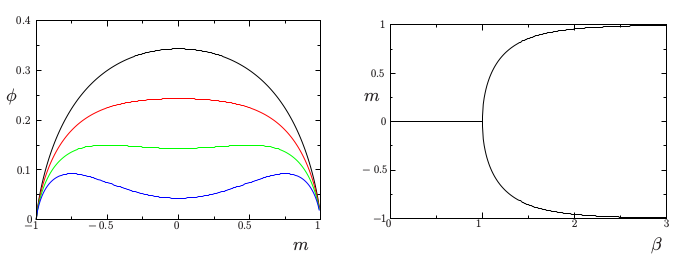
\includegraphics[width=\textwidth]{PhiPlots.png}
\caption{The plot on the left shows the variation of $\phi_{mf}(m;\beta,0)$ with $m$, for different values of $\beta$. For $\beta<1$, there is a unique maximum, and for $\beta>1$, there are two maxima---indicating a phase transition at $\beta=\beta_c=1$. On the right, the plot shows the variation of the values of $m$ that maximize $\phi_{mf}(m;\beta,0)$, with $\beta$. The phase transition at $\beta=1$ is indicated by a bifurcation.}
\end{figure}
\section{The Ising Spin-Glass (or Edwards-Anderson) Model}
In this section, we briefly go over yet another model for the interactions between particles. As before, $\bm{\sigma}\in \sX_{N} = \{-1,+1\}^{\mathbb{L}}$ represents a configuration of the $N$-particle system, with $\mathbb{L}=\{1,\ldots,L\}^{d}$ representing a $d$-dimensional lattice.
In the Ising spin-glass model,
\begin{equation*}
    E(\bm{\sigma}) = -\sum_{(ij)}J_{i,j}\sigma_i\sigma_j - B\sum_{i\in \mathbb{L}}\sigma_i.
\end{equation*}
Here, the first summation runs over each edge of the lattice, and the multiplying factor, $J_{i,j}\in \mathbb{R}$, for $i,j\in \mathbb{L}$. Note the difference in the energy function from the Ising model, in that now, each $2$-particle interaction is multiplied by a (possibly) different factor.
We state here that it is not straightforward to arrive at a low energy configuration in this model (by satisfying each local constraint), as elucidated in the example below:
\begin{shaded*}
\begin{exmp}
Consider the Ising spin-glass model, for an $L=2,\text{ }d=2$ system, with $B=0$. The lattice is hence a $2$-dimensional square, with vertices $V=\{(1,1),(1,2),(2,1),(2,2)\}$.
Let $J_{(1,1)\sim (1,2)}=1$, $J_{(1,1)\sim (2,1)}=1$, $J_{(2,1)\sim (2,2)}=1$ and $J_{(2,2)\sim (1,2)}=-1$, where the notation $(a,b)\sim (c,d)$ is used to represent the edge between $(a,b)$ and $(c,d)$, for $(a,b),(c,d)\in \mathbb{L}$. We observe that the two configurations,
\begin{align*}
    \bm{\sigma}^{1} &= \left(\sigma_{(1,1)}=1,\sigma_{(1,2)}=1,\sigma_{(2,1)}=1,\sigma_{(2,2)}=1\right)\\
    \text{and }\bm{\sigma}^{2} &= \left(\sigma_{(1,1)}=1,\sigma_{(1,2)}=-1,\sigma_{(2,1)}=1,\sigma_{(2,2)}=1\right)
\end{align*}
are degenerate, with $E(\bm{\sigma}^{1})=E(\bm{\sigma}^{2})=2$. This is, however, a \textbf{frustrated} system, since it is impossible to satisfy each local constraint induced by the individual $J_{i,j}$s, $i,j\in \mathbb{L}$.
\end{exmp}
\end{shaded*}
\section{Optimization and Statistical Physics}
Combinatorial optimization problems present inherent difficulties owing to the ``discreteness" (or lack of smoothness) of the space. In general, in such problems, given a configuration space $\sX$, we wish to find $C\in \sX$ with the smallest cost.
It is possible to introduce a Boltzmann probability distribution on the space of configurations as:
\begin{equation*}
    \mu_{\beta}(C) = \frac{1}{Z(\beta)}e^{-\beta E(C)},\quad Z(\beta) = \sum_{C\in \sX}e^{-\beta E(C)},
\end{equation*}
for $C\in \sX$. In the limit as $\beta\rightarrow \infty$, the probability distribution concentrates on the ground states---which is the case when all optimization constraints are satisfied.
We conclude the lecture with two different examples, to drive home the obstacles posed by such optimization problems:
\begin{shaded*}
\begin{exmp}(Min-Cuts on Graphs)
We consider again, the Ising spin-glass model, with $B=0$, and $E(\bm{\sigma})=\sum_{(ij)}J_{i,j}\sigma_i\sigma_j$.
Each configuration partitions the set $\{\sigma_1,\ldots,\sigma_N\}$ into $2$ subsets:
\begin{equation*}
    V_{+} = \{i:\sigma_i=+1\},\quad V_{-} = \{i:\sigma_i=-1\}.
\end{equation*}
Thus,
\begin{equation*}
    E(\bm{\sigma})=-C+2\sum_{(ij)\in \gamma(V_{+})}J_{i,j},
\end{equation*}
where $C=\sum_{(ij)}J_{i,j}$, and $\gamma(V_{+})=\{(i,j):i\in V_{+},j\in V_{-}\}$.
Solving for the lowest energy configuration, is hence, exactly equivalent to finding the min-cut in the graph \\$\sG=(V_{+}\cup V_{-},\sE)$, with $\sE$ being the set of edges induced by the particle interactions.
\end{exmp}
\end{shaded*}
\begin{shaded*}
\begin{exmp}(Error-Correcting Codes)
In this example, we illustrate the potential hardness of the decoding problem, for binary codes.

Recall the setting of a communication system, which consists of an encoder $e:m\in \{0,\ldots,2^{M}-1\}\mapsto \mathbf{x}\in\{0,1\}^{N}$, that maps the output of an i.i.d. uniformly distributed source, to a codeword $\mathbf{x}$. Let $\mathbf{y}\in \{0,1\}^{N}$ be the output of the channel described by the conditional distribution, $Q(\mathbf{y}|\mathbf{x})$, for $\mathbf{y},\mathbf{x}\in \{0,1\}^{N}$.

The decoder, $d:\mathbf{y}\in \{0,1\}^{N}\mapsto \mathbf{\hat{x}}\in \{0,1\}^{N}$, outputs an estimate, $\mathbf{\hat{x}}$, of the codeword $\mathbf{x}$. The average probability of error,
\begin{equation*}
    P_B^{avg} = \frac{1}{2^M}\sum_{m}\sum_{\mathbf{y}:d(\mathbf{y})\neq \mathbf{e(m)}}Q(\mathbf{y}|\mathbf{e(m)}) = 1 - \frac{1}{2^M}\sum_{m}\sum_{\mathbf{y}:d(\mathbf{y})= \mathbf{e(m)}}Q(\mathbf{y}|\mathbf{e(m)}).
\end{equation*}
It is, therefore, obvious (after interchanging summations) that the optimal decoder (that minimizes $P_B^{avg}$) must map the received word $\mathbf{y}$ to that codeword, $\mathbf{\hat{x}}$, that maximizes $Q(\mathbf{y}|\mathbf{\hat{x}})$.\\
However, one can note that this procedure of finding the ``most likely" codeword, involves searching over all possible $2^M$ codewords, leading to exponential time complexity. In fact, the general problem of decoding codes that admit a concise specification (polynomial in the block-length) is NP-hard.
\end{exmp}
\end{shaded*}
\end{document}